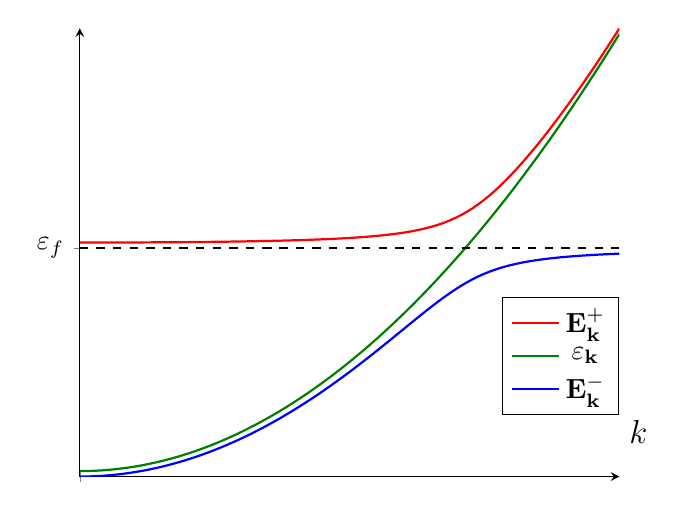
\begin{tikzpicture}
\begin{axis}[
    legend style={at={(1,0.4)}},
    ytick = {1},
    yticklabels = {$\varepsilon_f$},
    xtick = {0},
    xticklabels ={,,},
    xlabel = \large $k$,
    axis lines = left,
    x label style={at={(axis description cs:1,0.1)}, anchor = west},
    %y label style={at={(axis description cs:0.15,1)},rotate=-90,anchor=south},
    %xlabel = $x$,
    %sylabel = {$f(x)$},
]
%Below the red parabola is defined
\addplot [
    thick,
    domain=0:1.4, 
    samples=100, 
    color=red,
]{1/2 * (1 + x^2 + sqrt((x^2 - 1)^2 + 0.1))};


\addplot [
    thick,
    domain=0:1.4, 
    samples=100, 
    color=green!50!black,
]{x^2};

%Here the blue parabloa is defined
\addplot [
    thick,
    domain=0:1.4, 
    samples=100, 
    color=blue,
    ]{1/2 * (1 + x^2 - sqrt((x^2 - 1)^2 + 0.1))};


\addplot[
    thick,
    domain = 0:1.4,
    samples = 100,
    dashed
    ]{1};

\addlegendentry{$\mathbf{E_k^+}$}
\addlegendentry{$\mathbf{\varepsilon_k}$}
\addlegendentry{$\mathbf{E_k^-}$}
\end{axis}
\end{tikzpicture}